\section{Obecně}
Jak již bylo v textu této práce několikrát zmíněno, PhoneGap je v současné době pravděpodobně nejpoužívanější a nejznámější hybridní framework. Vývojáři se na svém webu chlubí, že zaznamenali již více než milion stažení jejich produktu a zároveň tvrdí, že je v současné době používán více než 400 000 vývojáři pro tvorbu tisícovek aplikací.

PhoneGap umožňuje vývojářům využívat při tvorbě mobilních aplikací webové technologie HTML5, CSS3 a JavaScript a zároveň jim prostřednictvím vlastního JavaScriptového API poskytuje možnost komunikace s operačním systémem a využití jeho nativních součástí, jako je například fotoaparát, akcelerometr nebo například výběr ze seznamu kontaktů. To vše multiplatformně.

V rámci této kapitoly již nebudu zabíhat do technických detailů vlastního fungování frameworku PhoneGap. Tuto oblast jsem již dostatečně pokryl v předchozí kapitole \ref{Chap:HybridniFrameworky}.\\ \\

\textit{\uv{Konečným cílem PhoneGap je, aby PhoneGap již nemusel existovat.} \cite{how_cordova_becomes_phonegap}}
\footnote{“The ultimate purpose of PhoneGap is to cease to exist.” \cite{how_cordova_becomes_phonegap}} \\

Skupina vývojářů stojící za PhoneGap uvádí, že za jejich prací stojí následující dvě kréda:

\begin{enumerate}
	\item Web vyřešil problém přenositelnosti.
	\item Každá technologie zastará.
\end{enumerate}

S prvním krédem se dá polemizovat jen velmi těžko. Program, umožňující zobrazovat webové stránky, najdeme dnes skutečně téměř na každé platformě. Co se ne zcela povedlo Javě, se webovým technologiím daří a jejich význam roste. Ne náhodou dnes používáme mnohem více webových aplikací než dříve a spousta aplikací, u kterých to bylo dříve nemyslitelné, se přesunula do cloudu a přistupujeme k nim přes webový prohlížeč. Jedním z nejzářnějších příkladů jsou například Google Dokumenty, které přispěly i k tvorbě této práce.

Krom těchto dvou kréd uvádějí vývojáři i dva cíle, ke kterým by jejich snažení mělo přispět:

\begin{enumerate}
	\item Vylepšit web (webové standardy), aby se stal prvotřídní vývojovou platformou.
	\item Docílit takového stavu webových standardů, aby byl PhoneGap zbytečný.
\end{enumerate}

Je pravdou, že různé týmy uvnitř konsorcia W3C pracují na vytvoření standardů, které umožní přístup k nativním funkcím telefonního přístroje přímo z prohlížeče bez použití jakékoliv mezivrstvy. Typickým příkladem realizace těchto snah je například standard pro využití geolokace, který již byl moderními prohlížeči implementován a je využit i v rámci PhoneGap, kde API volání pro geolokaci nedělá nic jiného, než že volá tuto standardizovanou funkci prohlížeče. Že cíle, které si tým kolem PhoneGap vytyčil, nejsou řečmi do větru, dokládá i fakt, že vývojáři stojící za tímto frameworkem jsou součástí právě těch skupin v rámci konsorcia W3C, které se starají o implementaci příslušných standardů.

\subsection{Licence}
Poté co byla firma Nitobi, která za PhoneGap původně stála, odkoupena společností Adobe, byl kód pohánějící framework PhoneGap věnován organizaci Apache Software Foundation pod názvem Apache Cordova. Nyní je tedy šířen pod licencí Apache License, Version 2. Tato licence nadále zaručuje otevřený přístup k vývoji na projektu i k použití samotného kódu.

\subsection{PhoneGap vs. Apache Cordova}
Zejména u lidí, kteří se s PhoneGap teprve seznamují, koluje mnoho nejasností ohledně rozdílu mezi PhoneGap a jeho dvojčetem Apache Cordova. Myslím, že stojí za to na tomto místě tyto nejasnosti ozřejmit.

Apache Cordova je jádro frameworku spravované Apache Software Foundation (ASF), na jehož základě je postavený framework PhoneGap. Dalo by se říci, že PhoneGap je distribucí Apache Cordova podobně, jako je operační systém Ubuntu distribucí, kterou pohání jádro Linux. Vývojáři PhoneGap nadále doplňují Apache Cordova o nové funkce a opravují nalezené chyby. K oddělení došlo zejména proto, že postupem času se dá očekávat hlubší integrace PhoneGap s nástroji Adobe, což by nebylo vhodné pro masové použití \cite{cordova_name}. 

PhoneGap není jedinou distribucí Apache Cordova, ve skutečnosti jí dnes implementuje do svých nástrojů mnoho firem, jako je například Salesforce nebo Facebook \cite{cordova_name}. Na vývoji Apache Cordova se nepodílí jen vývojáři PhoneGap, ale také mnoho dalších firem jako je například IBM či Microsoft.

\section{Historie}
\textit{\uv{Měli jsme v hlavě jen jeden cíl. Umožnit webovým aplikacím využívat nativní funkce iPhone.} \cite{phonegap_announcement}}
\footnote{“We went down with one goal in mind and that was to make native iPhone features available to web apps.” \cite{phonegap_announcement}} \\

Pojďme se stručně seznámit s historií PhoneGap a změnami, které vedly k frameworku, jak jej známe dnes. PhoneGap vznikl v roce 2008 na vývojářské akci iPhoneDevCamp, kde vývojáři firmy Nitobi přišli s nápadem, kterak umožnit vývojářům webových aplikací pro systém iOS (tehdy ještě iPhone OS) využívat některé oblíbené nativní funkce přístroje iPhone. V soutěži na iPhoneDevCamp sice PhoneGap neuspěl, to však firmu Nitobi nezastavilo v dalším rozvíjení svého nápadu.

V počátku své existence podporoval PhoneGap pouze systém iOS, ale multiplatformnost byla brána vývojáři na zřetel od samého počátku, a tak rychle přibyla podpora pro Android a BlackBerry. Nedlouho poté (v roce 2009) následovala podpora pro Symbian a Palm (webOS).

K začátkům frameworku PhoneGap se datuje série nepříjemností, které vznikly při schvalovacím procesu ze strany Applu, kdy Apple odmítal schvalovat a vpouštět na své oficiální tržiště aplikace napsané pomocí frameworku PhoneGap. Důvodem pro zamítání aplikací bylo porušení podmínek, které aplikace v AppStore musí splňovat. Aplikace napsané ve PhoneGap byly penalizovány, protože při jejich vývoji byl použit externí framework, což tyto podmínky zapovídají. Celá záležitost byla vyřešena domlouvou mezi vývojáři kolem frameworku PhoneGap a Applem, kdy byla stanovena „bezpečná verze“ frameworku PhoneGap (PhoneGap 0.8.0), jejíž použití bylo Applem oficiálně posvěceno a k aplikacím využívajícím tuto „bezpečnou verzi“ bylo během schvalovacího procestu přistupováno stejně jako k běžným nativním aplikacím. \cite{open_letter_to_apple,updates_on_apple,phonegap_permitted_appstore,phonegap_store_approval}

Multiplatformní záběr se stal zas o něco širším, když v roce 2010 přidal PhoneGap podporu pro Windows Phone 7 a také kvůli přechodu BlackBerry na WebKit, v šesté verzi svého operačního systému, byla podpora pro BlackBerry rozštěpena na dvě větve.

V listopadu 2010 Nitobi představilo v poloveřejné betě nástroj PhoneGap Build. Tento nástroj si podrobněji popíšeme později v této kapitole, teď jen zmíním, že se jedná o cloudovou službu, která umožňuje po nahrání zdrojových kódu vygenerovat instalační balíčky pro více platforem najednou. Vývojář tak nemusí pro každou platformu instalovat její SDK a generování binárních souborů provádět ručně. \cite{announcing_phonegap_build_beta} 

Pokračující růst PhoneGap dokládá i obliba, které se této framework těšil pouhé dva roky po svém vzniku. V listopadu 2010 zaznamenal PhoneGap již 350 000 stažení. S touto vzrůstající oblibou začalo Nitobi (původně konzultantská firma zabývající se tvorbou webů a JavaScriptových knihoven) na PhoneGap stále více sázet ve své obchodní strategii. Nejenže s ním pracovala ve své konzultantské činosti a doporučovala jeho používání svým zákazníkům, ale v únoru 2011 zavádí i placenou podporu pro vývojáře ve PhoneGap, v rámci které jim poskytuje webináře, přístup na privátní forum a pomoc v rámci office hours.

Dalším znakem úspěchu PhoneGap je i jeho adopce softwarovými giganty jako je Adobe či IBM, které začali tento framework integrovat do svých nástrojů, jako je Adobe DreamWeaver či IBM Worklight \cite{phonegap_worklight_enterprise,dreamweaver_supports_phonegap}. 

Prvním velkým milníkem pro PhoneGap bylo vydání verze 1.0.0, ke kterému došlo 29. 7. 2011. V té době PhoneGap již podporoval i platformu Samsung Bada a samotný framework zaznamenal 600 000 stažení s průměrem kolem 40 000 stažení měsíčně. \cite{phonegap_1_released} 

V září 2011 se PhoneGap Build přesouvá do veřejné betaverze a zároveň byly zveřejněny cenové plány pro jeho použití. Ty se pohybovali od \$0 pro vývoj open-source aplikací po \$900 ročně pro vývoj komerčních aplikací s uzavřeným kódem. \cite{phonegap_build_open_beta}

3. září 2011 Nitobi na svém blogu oznámilo, že uzavřelo dohodu o svém převzetí firmou Adobe \cite{nitobi_adobe1}. \\

\textit{\uv{PhoneGap je perfektním doplněním široké palety nástrojů pro vývojáře od společnosti Adobe (včetně Adobe AIR) a dovolí nám nadále poskytovat vývojářům ta nejlepší a nejmodernější řešení pro vytváření inovativních aplikací napříč platformami a zařízeními.}} Danny Winokur, Adobe \cite{nitobi_adobe1}
\footnote{“It’s a perfect complement to Adobe’s broad family of developer solutions, including Adobe AIR, and will allow us to continue to provide content publishers and developers with the best, cutting-edge solutions for creating innovative applications across platforms and devices.” Danny Winokur, vice president and general manager, Plat-
form, Adobe \cite{nitobi_adobe1}}\\

V rámci tohoto převzetí Nitobi oznámilo, že věnuje zdrojové kódy frameworku PhoneGap organizaci Apache Software Foundation (ASF) pod názvem Apache Callback, který byl později změněn na Apache Cordova \cite{nitobi_adobe2,phonegap_13_released}. 

Akvizice Nitobi firmou Adobe se podařila úspěšně dokončit 27. října 2011 \cite{nitobi_adobe2}. Analytici se shodují, že hlavním smyslem této akvizice byla snaha Adobe posílit svojí pozici na poli vývoje aplikací v HTML5, protože jeho vlastní technologie Flash je (zvlášť v mobilním světě) na ústupu. Očekávalo se začlenění PhoneGap do vývojářských nástrojů, které Adobe poskytuje webovým vývojářům.

Nehledě na tuto velkou změnu popularita PhoneGap dále pozvolna stoupala a v červnu roku 2012 dosahoval průměrný měsíční počet stažení hodnoty 100 000 \cite{phonegap_myths}.

20. července 2012 byla oficiálně uvolněna verze 2.0, která (krom jiného) přinášela také Cordova WebView, což je možnost použití WebView v rámci nativní aplikace současně se všemi výhodami PhoneGap. Dále přibylo také mnoho vylepšení command-line interfacu, které umožňuje ovládat PhoneGap z konsole. \cite{phonegap_2_released} 

V září 2012 byl oficiálně spuštěn PhoneGap Build, který je nyní dostupný ve stabilní verzi \cite{phonegap_build_launched}. Zároveň byla v listopadu 2012 vydána verze 2.2.0, která přináší podporu Windows 8 v rámci PhoneGap. V době psaní této práce se framework nachází ve verzi 2.5.0. Vydání verze 3.0.0 je naplánováno na červenec 2013 \cite{cordova_roadmapprojects}. 

\subsection{Ocenění}
PhoneGap se za dobu své existence dočkal celé řady ocenění od všemožných institucí.

\begin{enumerate}
	\item 2009: People’s Choice award v rámci Web 2.0 Expo LaunchPad competition \cite{phonegap_winning_webexpo}
	\item 2012: Best Cross-Platform Development Tool by CodeProject \cite{phonegap_best_xplatfrom_tool}
	\item 2012: Technology of the Year By InfoWorld \cite{infoworld_technology_of_2012}
	\item 2012: “Champion” by Info-Tech Research Group v rámci 2012 Vendor Landscape: Mobile Development Platforms \cite{phonegap_champion}
	\item 2012: Best Mobile Development Tool by Dr. Dobb's Jolt Awards \cite{phonegap_best_mobile_dev_tool}
\end{enumerate}

\section{Vývojářské nástroje}
\subsection{Vývoj}
Na začátku této sekce krátce pohovořím o nástrojích, které můžeme pro vývoj ve PhoneGap využít. Před vznikem cloudové služby PhoneGap Build byl vývoj, zvláště pokud jste chtěli aplikaci cílit na více platforem, poměrně kostrbatý. To bylo zapříčiněno několika faktory:

\begin{enumerate}
	\item Různá SDK pro sestavení nativních binárních souborů;
	\item Různá adresářová struktura projektů pro jednotlivé platformy;
	\item Odlišné JavaScriptové knihovny (PhoneGap) pro jednotlivé platformy;
\end{enumerate}

V důsledku to znamenalo, že pro vývoj aplikace pro systém Android jste si museli stáhnout Eclipse a Android SDK a vývoj vést v těchto nástrojích. Pokud jste následně chtěli aplikaci portovat na iOS, znamenalo to stažení iOS SDK a Xcode (funguje pouze na systému Mac OS), úpravu adresářové struktury projektu a využití knihovny PhoneGap určené pro systém iOS.

Díky cloudovému nástroji PhoneGap Build (podrobněji si ho popíšeme níže v této kapitole) se vývoj aplikací ve PhoneGap výrazně usnadnil a to zejména při cílení na více platforem. Jelikož PhoneGap Build potřebuje k vygenerování nativních binárních souborů pouze samotné zdrojové kódy aplikace, nemusí se vývojář zabývat ani jedním z výše vyjmenovaných problémů.

Pokud vývojář není závislý na SDK konkrétní platformy, může pro vývoj použít prakticky libovolný nástroj. Může zůstat u mohutného IDE, jako je např. Eclipse nebo využít svůj oblíbený textový editor (TextMate, gedit, Sublime Text apod.).

\subsection{Rozšíření}
Pokud vyvíjíme pro konkrétní platformu nebo chceme jen přidat některé specifické funkce, které PhoneGap nativně nenabízí, můžeme sáhnout do poměrně bohaté sbírky rozšíření, která vznikla v rámci komunity, ale je oficiálně spravována projektem PhoneGap na adrese \url{https://github.com/purplecabbage/phonegap-plugins}. % TODO vylepšit URL

Najdeme tu bohatou sbírku pluginů, které pokrývají širokou škálu funkcí. Můžeme si některé z nich uvést:

\begin{enumerate}
	\item InAppPurchaseManager (iOS)
	\item BarcodeScanner
	\item GoogleAnalytics
	\item PDFViewer
	\item Twitter
	\item iCloudKV (iOS)
	\item Bluetooth
	\item NFC
	\item PayPalPlugin
\end{enumerate}

Pluginy se používají podobným způsobem jako samotný framework. Konkrétní plugin se vloží do projektu a jeho funkce jsou následně volány z JavaScriptového kódu vlastní aplikace. Logicky je nutné počítat s tím, že použití takového pluginu silně ochromí přenositelnost celé aplikace a před provedením portu bude třeba provést odpovídající úpravy.

\subsection{Debugování a testování} \label{Sec:DebugaTest}
\subsubsection{Testování}
V průběhu celého vývoje aplikace je třeba neustále testovat a ověřovat její funkčnost v prostředí co možná nejbližším produkčnímu. Pro tento účel poskytují tvůrci jednotlivých platforem simulátory (emulátory), které simulují běh aplikace v rámci daného operačního systému či dokonce přímo v rámci konkrétního zařízení.

V případě testování není žádný rozdíl mezi nativními aplikacemi a těmi hybridními napsanými ve PhoneGap. Vývojář nahraje svojí aplikaci do simulátoru a zkouší její funkčnost. To samé se týká testování aplikace na reálném zařízení, které by mělo být součástí každého vývojového plánu.

\subsubsection{Debugování}
Při vývoji čistě nativních aplikací využívá vývojář pro ladění svých aplikací debugovací nástroje, které mu poskytuje SDK a další nástroje konkrétní platformy. Problém s těmito nástroji je, že většinou nejsou připravené na ladění kódu psaného webovými jazyky. To staví vývojáře do poměrně nepříjemné pozice, kdy jsou buď nuceni protkat svůj kód voláním funkce alert() či console.log(), které používají pro vypsání ladících výpisů nebo využít některého z nástrojů třetích stran, které jsou na ladění hybridních aplikací připraveni. Dva takové nástroje si nyní uvedeme.

\paragraph{Ripple Mobile Enviroment Emulator}
Ripple Mobile Enviroment Emulator (RMEE) je náhrada klasického emulátoru z SDK jen s tím rozdílem, že je velmi odlehčený a běží jako rozšíření ve webovém prohlížeči Google Chrome či Chromium. RMEE narozdíl od holého webového prohlížeče dokáže nasimulovat i volání nativních funkcí frameworkem PhoneGap a je tak velice vhodným nástrojem pro rychlé testování mobilních aplikací bez nutnosti zdlouhavě nahrávat aplikaci do emulátoru nebo vlastního fyzického zařízení.

Výhodou použití RMEE je, že dává vývojáři k dispozici krom samotného emulátoru i veškeré vývojářské nástroje prohlížeče Google Chrome, které se používají pro ladění webových aplikací. Může tak za běhu upravovat některé parametry své aplikace a pohodlně tak ladit vlastní aplikaci.

\begin{figure}\centering
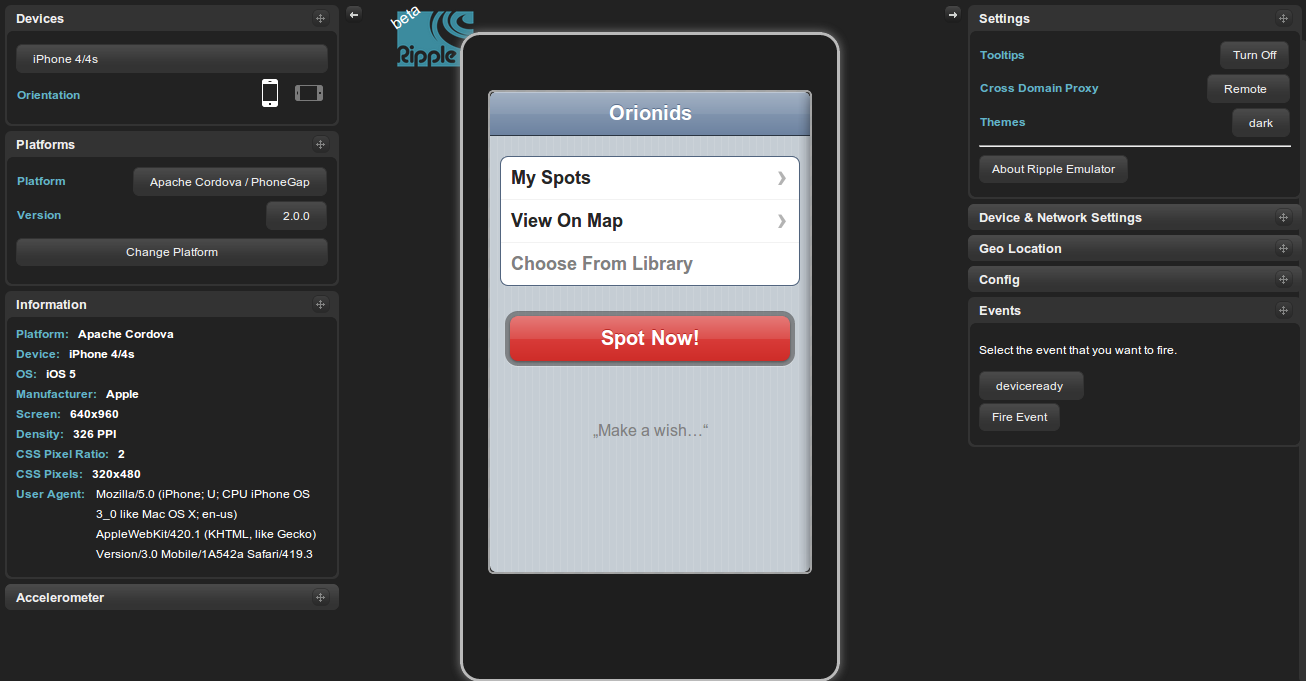
\includegraphics[width=0.9\textwidth]{RMEE.png}
\caption{Ripple Mobile Enviroment Emulator}
\label{fig:RMEE}
\end{figure} 

Je jasné, že RMEE nenahradí testování v klasickém emulátoru či dokonce na fyzickém zařízení, neboť zdaleka nedokáže emulovat veškerá specifika hostitelských operačních systémů, ale stále je poměrně vhodným nástrojem pro rychlé testování aplikace zvláště v rané fázi vývoje.

RMEE je dostupný z adresy \url{http://emulate.phonegap.com}

\paragraph{Web Inspector Remote}
Web Inspector Remote neboli Weinre je ladící nástroj trochu jiného druhu. Nezabývá se emulací běhu aplikace, ale funguje jako vzdálený ladící nástroj. Jeho použití je poměrně jednoduché. Do kódu své aplikace vložíte skript umístěný na vzdáleném serveru (\url{http://debug.phonegap.com}) s unikátním označením své aplikace.

\begin{lstlisting}[language=HTML,breaklines=true]
<script src="http://debug.phonegap.com/target/target-script-min.js#myapp"></script>
\end{lstlisting}

Samotné debugování probíhá v prohlížeči, do kterého vývojář zadá adresu serveru s identifikátorem laděné aplikace \url{http://debug.phonegap.com/client/\#myapp}. Vývojáři je k dispozici JavaScriptová konzole a další nástroje pro ladění webových aplikací.

\subsection{Sestavení a publikace}
Pokud již máme aplikaci vytvořenou a důkladně otestovanou, je na řadě její sestavení a případná publikace například na oficiálním tržišti s aplikacemi. Za účelem sestavení aplikace nám PhoneGap umožňuje jít dvěma cestami. První z nich je sestavení nativního instalačního balíčku s využitím SDK konkrétní platformy vhodný k odeslání na tržiště. Toto je klasická cesta a je vhodná, pokud cílíme pouze na jednu platformu. Problém nastává, pokud chceme vytvořit balíčky pro více platforem najednou. Jak jsem již zmínil výše, v takovém případě jsme nuceni stáhnout SDK každé jednotlivé platformy, náš projekt upravit a poté s pomocí SDK vytvořit nativní binární soubor. Že toto není dobrý způsob, si uvědomovali i tvůrci frameworku PhoneGap a proto již v počátku ve svých úvahách počítali s cloudovým nástrojem, který sestavování aplikací značně usnadní.

\subsubsection{PhoneGap Build} \label{Sec:PhoneGapBuild}
PhoneGap Build je nástroj dostupný z adresy \url{http://build.phonegap.com}. Umožňuje nám z jednoho místa a z jednoho zdrojového kódu vytvořit v jednom čase instalační balíčky pro platformy iOS, Android, Windows Phone, BlackBerry, webOS a Symbian.

Pojďme si v krátkosti popsat jak celý systém funguje. Vývojář je na začátku vyzván k propojení PhoneGap Build se svým účtem na Githubu, na němž má ve veřejném repozitáři umístěny zdrojové kódy své aplikace. Poté se dostane do ovládacího panelu, kde vybere z nabídky správný repozitář, ve kterém se PhoneGap Build pokusí najít soubor index.html. Jakmile se mu to podaří, nabídne vývojáři možnost si vygenerovat instalační balíčky pro jednotlivé platformy pomocí jednoho kliknutí. Vyhotovení balíčků trvá několik vteřin a poté jsou uživateli k dispozici ke stažení.

\section{API} \label{Sec:API}
Hlavním důvodem, proč vývojáři sahají po použití frameworku PhoneGap, je sada JavaScriptových API, pomocí které zprostředkovává komunikaci mezi webovou aplikací a operačním systémem na daném zařízení. Pojďme si nyní stručně popsat jednotlivá API volání.

\subsection{Accelerometer}
Akcelerometr se používá ke zjištění orientace daného přístroje. Hojně je využíván například v hrách, kde hráč ovládá hru pomocí naklopení telefonu.

Tento objekt obsahuje sadu metod, které umožňují vrátit současnou polohu přístroje pomocí trojice souřadnic x, y a z. Je také možné nastavit sledování změn polohy v zadaném intervalu.
Umožňuje zrušit sledování změn vyvolané předchozí metodou.

\subsection{Camera}
Sada funkcí sloužící pro přístup k fotoaparátu mobilního zařízení. Umožňuje pořízení fotografie z daného zdroje. Zdroj je specifikován ve volání funkce getPicture, může se jednat buď o pořízení nového snímku nebo o vybrání již pořízeného snímku z fotoalba. Fotografie je vrácena buď jako URI nebo jako String zakódovaný v base64.

\subsection{Capture}
API umožňující zachycení videa, audia či fotografie. Funguje tak, že otevře výchozí aplikaci pro pořízení daného média a vrátí zpět informace o pořízených záznamech jako URI.

\subsection{Compass}
Sada metod umožňující rozpoznat, jakým směrem je zařízení namířeno. Zavoláním funkce getCurrentHeading získáme informace o aktuální orientaci zařízeni vzhledem ke světovým stranám ve stupních od 0 do 359,99. Údaje o orientaci přístroje můžeme také snímat v pravidelném intervalu pomocí funkce watchHeading.

\subsection{Connection}
Connection je objekt, který uchovává informace o připojení daného zařízení. Umožňuje vývojáři rychle zjistit, zda je telefon připojen k WiFi, 3G či kabelovému připojení, ale také dokáže ověřit, že přístroj není k internetu připojen vůbec.

\subsection{Contacts}
Metodami tohoto objektu může vývojář přistupovat k nativní databázi kontaktů v daném mobilním zařízení. Kontakt je možno v databázi buď vyhledat či vytvořit zcela nový pomocí funkce create.

\subsection{Device}
V objektu Device vývojář nalezne důležité informace o hardware a software daného zařízení. Obsahuje informace o názvu zařízení, aktuálně používané verzi PhoneGap, operačním systému a jeho verzi a také UUID identifikátor daného přístroje.

\subsection{Events}
V aplikaci často potřebujeme reagovat na události vyvolané přímo uživatelem nebo operačním systémem. PhoneGap nám to umožňuje pomocí sady předdefinovaných událostí. Vývojář může reagovat například na stisknutí tlačítka zpět, ztišení nebo zvýšení hlasitosti, přepnutí aplikace do pozadí a mnoho dalšího. V rámci tohoto API můžeme také rozpoznat, zda-li je zařízení připojeno k internetu nebo jaký je stav baterie v přístroji.

\subsection{File}
Sada objektů implementujících W3C specifikaci API pro zápis, čtení a navigaci v nativním filesystému. Soubory či složky můžeme vytvářet, procházet, kopírovat, mazat apod.

\subsection{Geolocation}
API umožňující přístup k informacím o zeměpisné délce a šířce daného zařízení. Tyto informace mohou pocházet buď z GPS modulu nebo z jiných zdrojů jako například IP adresa či GSM připojení. Informace o poloze můžeme získat buď jednorázově či je snímat v pravidelném intervalu, což se může hodit například pro turistické či fitness aplikace.

\subsection{Globalization}
Objekt globalization obsahuje informaci o preferovaném jazyce, nastavené časové zóně a podobně.

\subsection{InAppBrowser}
Internetový prohlížeč, který se otevře v rámci aplikace po zavolání metody window.open. API nám umožňuje naslouchat událostem ze synovského prohlížeče a regovat na ně.

\subsection{Media}
Pomocí objektu Media může vývojář zajistit nahrávání a přehrávání audio souboru. Objekt obsahuje rozmanité funkce, můžeme například získat aktuální pozici v právě přehrávaném souboru, zjistit jeho délku, posunout se v něm apod. Nechybí ani standardní metody pro spuštění nebo zastavení přehrávání či nahrávání.

\subsection{Notification}
Umožňuje upozornit uživatele pomocí různých druhů notifikací. Příkladem upozornění může být vibrace, alert box nebo pípnutí.

\subsection{Splashscreen}
Pomocí tohoto API může vývojář ovlivnit zobrazování splashscreenu při startu aplikace.

\subsection{Storage}
API založené na W3C specifikaci umožňující ukládání dat do lokální databáze. Metoda openDatabase vytvoří nový objekt Database, nad kterým můžeme provádět transakce pomocí metody executeSql objektu SQL Transaction.

\subsection{Tabulka podpory API volání v rámci platforem}
Jednotlivá API volání bohužel nejsou podporována konzistentně napříč platformami. V následující tabulce najdete přehled podpory jednotlivých volání napříč mobilními platformami.

\section{PhoneGap v reálných aplikacích}
Pokud jsme dosud slyšeli jen čísla, kolikrát byl PhoneGap stažen, je čas se přesvědčit, že jej vývojáři opravdu využívají při reálném vývoji masově rozšířených aplikací. Vybral jsem 3 nejzajímavější aplikace, při jejichž vývoji byl využit PhoneGap.

\subsection{Wikipedia}
Otevřená encyklopedie Wikipedia používá PhoneGap pro vývoj oficiální mobilní aplikace, přes kterou mohou uživatelé vyhledávat, zobrazovat a ukládat jednotlivé články z nejobsáhlejší encyklopedie světa. Aplikace je v současnosti portována na platformách iOS, Android a BlackBerry Playbook.

% \begin{figure}[H]\centering
% 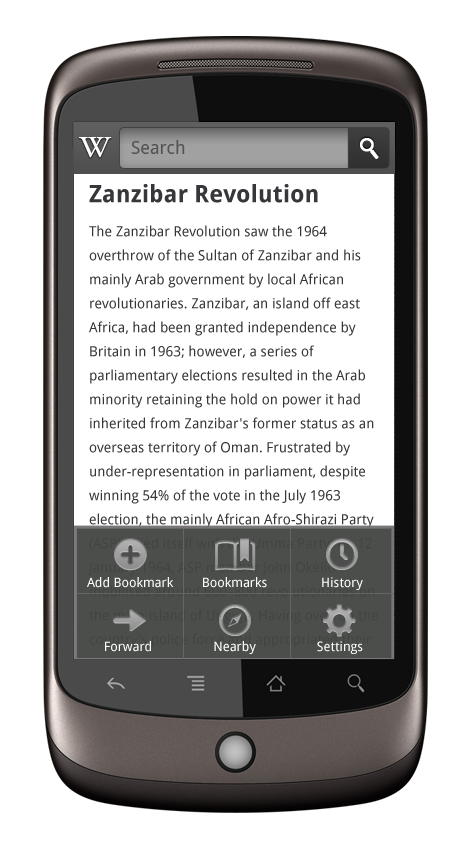
\includegraphics[width=0.4\textwidth]{wikipedia.png}
% \caption{Aplikace Wikipedia na OS Android \cite{google_android_wikipedia}.}
% \label{fig:WikipediaApp}
% \end{figure} 

\subsection{BBC Olympics}
Pro účely letních olympijských her v Londýně v létě 2012 vznikla pro britskou veřejnoprávní televizi BBC aplikace, která umožnila uživatelům přísun čerstvých novinek z dění na sportovištích. Aplikace nabízela například živé videopřenosy ze všech sportovišť, živý textový komentář k jednotlivým sportům, sestřihy toho nejlepšího, možnost čtení nejzajímavějších článků offline a mnoho dalšího. \cite{phonegap_bbc_olympics_app}

BBC Olympics byla dostupná na třech platformách – iOS, Android a Blackberry.

% \begin{figure}\centering
% 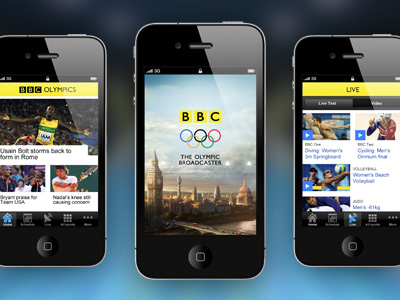
\includegraphics[width=0.5\textwidth]{bbc.jpg}
% \caption{Aplikace BBC Olympics na platformě iOS \cite{dribbble_bbc_olympics}.}
% \label{fig:BBCApp}
% \end{figure} 

\subsection{Fruit Salad}
Fruit Salad je hra, kde se hráč snaží skládat pod sebe stejné druhy ovoce a získávat za to body. Tato hra vytvořená pomocí HTML5 je dostupná pro platformu Android.

\textit{\uv{PhoneGap Build je skvělý nástroj pro webové vývojáře, kteří chtějí zveřejnit své HTML aplikace na App Store.}} \cite{phonegap_fruit_salad}
\footnote{“PhoneGap Build is a great tool for web developers who want to give App Store visibility to their HTML apps” said Fruit Salad creator, Baptiste Brunet. \cite{phonegap_fruit_salad}} \\

% \begin{figure}\centering
% 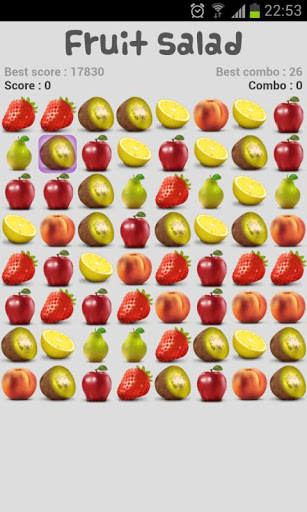
\includegraphics[width=0.4\textwidth]{fruitsalad.jpg}
% \caption{Hra Fruit Salad běžící na OS Android \cite{phonegap_fruit_salad}.}
% \label{fig:FruitSalad}
% \end{figure} 

\section{Budoucnost}
Co očekávat od budoucích let v souvislosti s PhoneGap? Jednoznačně mnohem hlubší integraci s Adobe produkty. Ačkoliv se to již u některých produktů (Adobe DreamWeaver) stalo, od převzetí PhoneGap firmou Adobe se očekávalo v tomto ohledu mnohem více. V dalších letech tak můžeme očekávat zařazování PhoneGap do vývojářských nástrojů, které Adobe poskytuje vývojářům HTML5 aplikací.

Jak jsem již předeslal na začátku této kapitoly, cílem Phonegap je, aby PhoneGap nebyl třeba. Za tímto účelem se vývojáři PhoneGap účastní tvůrčích skupin v rámci konsorcia W3C pro vytváření nových webových standardů. Jakmile budou nové standardy vytvořeny, dá se očekávat jejich rychlá implementace do PhoneGap, jako je tomu již nyní u API pro geolokaci nebo u lokálního úložiště dat.

Dalším cílem bude větší a pohodlnější rozšiřitelnost frameworku. Pluginy by mělo být možné lépe vyhledávat a snadněji instalovat. Pokročilejší vývojáře jistě potěší i plánované vylepšování řádkového interface, kterým je možno framework ovládat z konsole. Zároveň se plánuje velká revize celého API a jeho pročištění a další sjednocení. Jedním z velkých cílů je, aby bylo přidání podpory pro nové platformy co možná nejjednodušší.

Když je řeč o nových platformách, bylo by dobré zmínit, které jsou další na řadě. Vývojáři ve svých plánech hovoří zejména o dvou – Tizen a Firefox OS. Tizen je open-source operační systém pro široké spektrum zařízení vyvíjený pod záštitou Linux Foundation. O Firefox OS jsem hovořil již v kapitole \ref{Sec:FxOS}. Jedná se o mobilní operační systém od společnosti Mozilla postavený čistě na webových technologií pomocí W3C standardů a také Mozilla WebAPI.

Vydání PhoneGap ve verzi 3.0.0 je naplánováno na červenec 2013 \cite{cordova_roadmapprojects}.